\section{Applications}
The concept of dynamic demand-driven deployment is not new,
and has been used in various applications. Various algorithms
are used to optimize deployment of facility or utilization
of given sources.

To maximize fleet utilization and minimize
operating costs, airlines predict future demands
and optimize their flight schedules and aircraft
types using linear programming methods \cite{berge_demand_1993}. The demand
benefits and costs of ticket pricing, aircraft assignment, and crew 
scheduling are evaluated with a linear optimization method called
 ``Demand Driven Dispatch'' \cite{shebalov_practical_2009}, a type
of deterministic optimization method.

A sawmill facility that processes timber contains 
many steps, from sawing, drying to planning. An
agent-based simulation is used to analyse demand-
driven production planning for a manufacture facility
in Eastern Canada \cite{yanez_agent-based_2009}.
The facility unit can be represented by a group of many facilities,
for example, source, sawing operations, drying operations, warehouse,
make, and delivery. In the simulation, each agent is given its parameters
and model its procedures.

The demand agent communicates the demand plan, which are
order quantities for product needs at specific dates,
to the make agent of the demand plan,
which will cause the make agent to communicate to the source agent. Then the
analysed and planned supply chain will be moved back to the make agent and
to the deliver agent.

\begin{figure}
	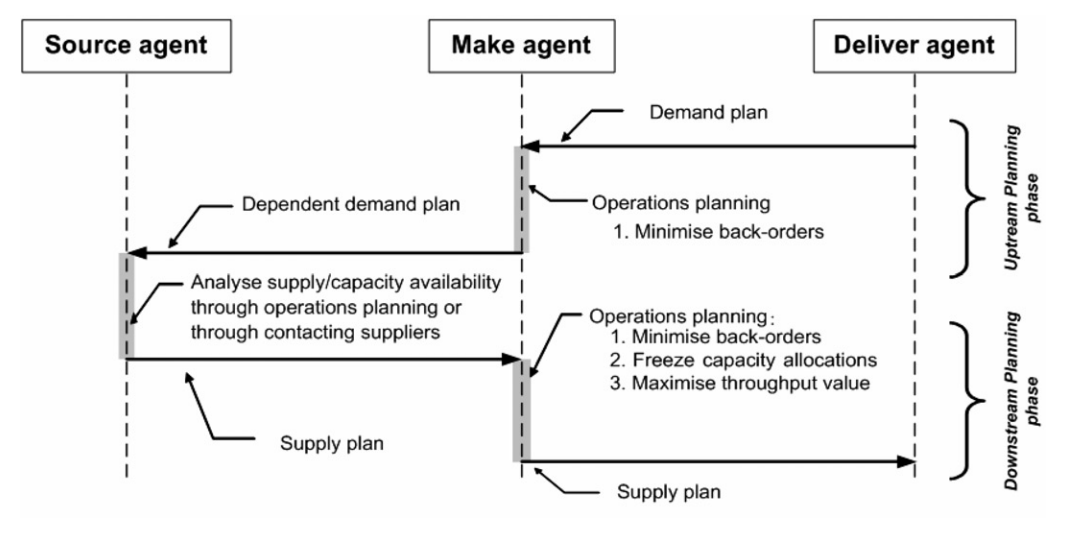
\includegraphics[width=\textwidth]{./images/timber_process.png}
	\caption{Agent Coordination Protocol \cite{yanez_agent-based_2009} } 
	\label{fig:timber_process}
\end{figure}


An intelligent building design minimizes 
the cost of operation by maximizing its efficiency,
especially in its energy utilization. In 
\cite{gonzalez_detailed_2002}, a feedback artificial neural
network method is used to predict future steam load from various
metrics, like input temperature, hour, and day.

Another paper \cite{kusiak_data-driven_2010} uses data-mining algorithms
to correlate steam load and weather data, and predicts
future steam load using the multiple-linear Perceptron ensemble
NN. The training set with 13 different parameters such as mean temperature,
and mean humidity are evaluated with its importance to predicting steam load.

